\section{Related Work}
Tarzan’s P2P network is much more secure than Boomerang, but may not function well in the Bitcoin environment due to scalability. Tarzan’s peer discovery protocol involves gossip and validation. Nodes gossip network information by exchanging all known addresses and corresponding public key hashes. A node validates an address by directly connecting to it with a gossip message that includes a nonce.

The benefit of Tarzan’s gossip procedure is that malicious nodes cannot respond with a different public key for every node in the network. Nodes learn public keys from gossip and not from the owner of the keys. Tarzan’s validation method prevents the propagation of invalid address information throughout the network. Assuming the first node a client connects to in the Tarzan network is honest, the client will eventually learn of every honest node in the network. The Tarzan network is not as scalable due to the amount of communication required to set up and maintain the network.

\begin{figure}[ht!]
\begin{center}
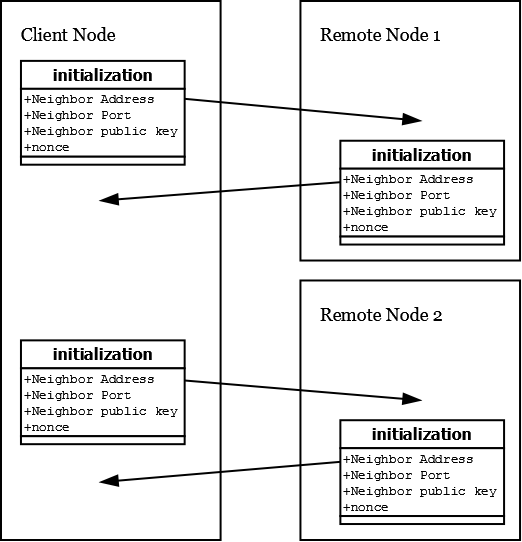
\includegraphics[scale=0.3]{./images/tarzan_protocol.png}
\caption{Tarzan gossip and validation protocol.}
\label{fig:tarzan_protocol}
\end{center}
\end{figure}

Peer-to-peer distributed hash table (DHT) networks, such as Chord and Kademlia, use a distributed system to keep track of key-value pairs. DHT networks use a 160-bit key space. The Chord network has the keys arranged in a circle. Each node in the Chord network maintains a segment of the circle adjacent to it. A successor to a Chord node is the node that maintains the next set of keys. By searching linearly through nodes, the node responsible for a key-pair can be found. To speed up searches, each node also keeps a “finger table” that contains successor information as shown below.

\begin{figure}[ht!]
\begin{center}
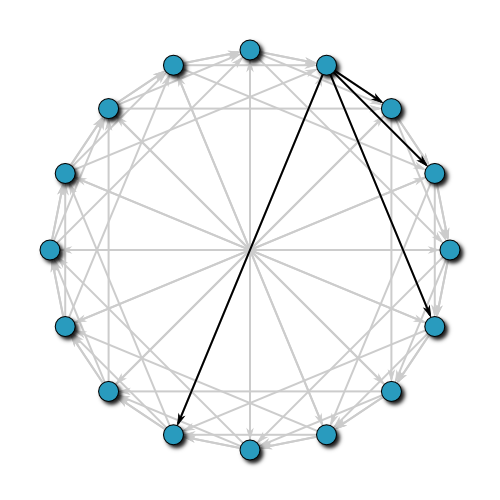
\includegraphics[scale=0.5]{./images/chord.png}
\caption{A Chord network with ``finger'' table entries highlighted.}
\label{fig:chord}
\end{center}
\end{figure}

Kademlia DHT is similar to Chord except that it is organized as a tree and distance is calculated using the “exclusive or” operation. The “exclusive or” operation allows the nodes in the Kademlia network to have symmetric distances between two nodes. Kademlia’s simpler distance calculation and iterative search, which is made possible by the tree-shaped network, allows for much faster searches than the Chord network. Both networks are decentralized, autonomous network that has fault tolerance and scalability. Unlike the Tarzan network, DHT networks do not prevent attacks on key searches or index poisoning and therefore allow a few malicious nodes to prevent nodes from finding other honest nodes.